        \documentclass{standalone}
        \usepackage{tikz}
        \usetikzlibrary{arrows}
        \usepackage{amsmath}
        \usepackage{amsfonts}
        \begin{document}
        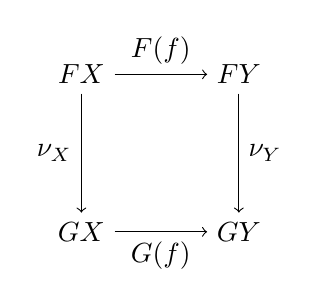
\begin{tikzpicture}

    \node at (0,0) (FX) {$FX$};
    \node at (2,0) (FY) {$FY$};
    \node at (0,-2) (GX) {$GX$};
    \node at (2,-2) (GY) {$GY$};
    \draw[->] (FX) -- node[above] {$F(f)$} (FY);
    \draw[->] (FX) -- node[left] {$\nu_X$} (GX);
    \draw[->] (GX) -- node[below] {$G(f)$} (GY);
    \draw[->] (FY) -- node[right] {$\nu_Y$} (GY);
        \end{tikzpicture}
        \end{document}
